\section{Introduction}
The fabrication of preforms for resin impregnation in composites are typically manufactured by deposition of a high number of slender textile yarns on the surface of a rigid body with complex geometry (mandrel). For the modelling of the yarn-to-mandrel contact interactions, the mandrel can either be modelled as a rigid body or as a beam for the specific case of a cylindrical geometry of mandrel. In the following numerical tests, both the cases have been studied. In the first test, a cylindrical shaped mandrel is modelled as a stocky and fixed beam, along with two slender textile yarns in contact with the mandrel. Further in the second test, the mandrel is modelled as a rigid body with contact-friction interactions modelled as beam-to-rigid body contact.

\section{Mortar contact for yarn-mandrel interactions}
\subsection{Test case description}
The fabrication of preforms for resin impregnation in composites are typically manufactured by deposition of a high number of slender textile yarns on the surface of a rigid body with complex geometry (mandrel). For the modelling of the yarn-to-mandrel contact interactions, the mandrel can either be modelled as a rigid body or as a beam for the specific case of a cylindrical geometry of mandrel. In this numerical test, a cylindrical shaped mandrel is modelled as a stocky and fixed beam, along with two slender textile yarns in contact with the mandrel.\\
The textile yarns are modelled as geometrically exact beams using the Lie group $SE(3)$ formalism presented in \cite{sonneville2014geometrically}. On deposition on mandrel surface, the contact forces are modelled either as concentrated point forces (for large contact angles) or distributed over a continuous patch (for acute contact angles). The mandrel is modelled as the master beam and the yarns as the slave beams. A Lagrange multiplier shall be used to denote the contact pressure, which is discretized using standard linear shape functions for first order interpolation. For the quasi-static case, the discrete equilibrium system is formulated presented in \cite{bosten2022mortar}:

\begin{subequations}
\begin{gather}
\boldsymbol{\mathrm{f}}^{\textrm{int}}(q) + \boldsymbol{\mathrm{B}}^{T}(q) \boldsymbol{\lambda} = \boldsymbol{\mathrm{f}}^{\textrm{ext}}(q)\\ \label{quasistatic}
\boldsymbol{\mathrm{0}} \leq \boldsymbol{\lambda} \perp \boldsymbol{\mathrm{g}}^{\textrm{con}} \geq \boldsymbol{\mathrm{0}} \label{LCP}
\end{gather}
\label{equilibrium}
\end{subequations}
where, Equation \ref{LCP} represents a linear complementarity problem (LCP) which is further solved using an augmented Lagrangian formulation. $\boldsymbol{\mathrm{f}}^{\textrm{int}}$ and $\boldsymbol{\mathrm{f}}^{\textrm{ext}}$ are internal and external force vectors respectively, $\boldsymbol{\mathrm{B}}$ is the constraint gradient, $\boldsymbol{\lambda}$ are the Lagrange multipliers and $q$ is the configuration variable, and $\boldsymbol{\mathrm{g}}^{\textrm{con}}$ is the weighted normal constraints. For element $e$, it is defined as: 

\begin{equation}
    \boldsymbol{\mathrm{g}}_e^{\textrm{con}}(q_e) = \int_{s^e_{a}}^{s^e_{b}} \boldsymbol{\mathrm{N}}^{T} g \, \mathrm{d}s_1
\end{equation}
which is defined on the slave beam ($s_1$) along with shape functions $\boldsymbol{\mathrm{N}}$ defined as $\boldsymbol{\mathrm{N}} (s_1) = \begin{bmatrix}
\frac{s_1}{L_{e_1}} & 1 - \frac{s_1}{L_{e_1}} 
\end{bmatrix}$. 

\subsection{Simulation setup}
A quasi-static frictionless simulation of two beams deposited on the surface of a stocky and fixed beam is performed using Odin multibody dynamics research code \cite{odin2022}. The radius of the slender beam is $r_y = 0.002$ m along with the length $l_y = 5$ m. Similarly, the radius of the stocky beam is $r_m = 0.2$ m along with length $l_m = 5$ m. The yarns and mandrel are discretized using 40 beam finite elements and the material properties of basalt fibres are assigned for the yarns as $E = 90$ GPa, $\nu = 0.21$ and $\rho = 2750$ Kg/m$^3$ and properties of steel assigned to the mandrel i.e. $E = 200$ GPa, $\nu = 0.3$ and $\rho = 7750$ Kg/m$^3$. A spherical joint is used at the starting positions of the slender beams to allow rotation. On the contrary, the stocky beam is fully constrained using a clamped essential boundary condition.\\

\subsection{Results}
The cross-winding of two yarns on the mandrel surface is shown in Figure \ref{testsetup}. For performing the test, a CSR Pardiso linear solver has been used along with a Newton nonlinear solver for which the maximum iterations is set to 100 and a relative tolerance of $1\mathrm{e}{-4}$ as presented in the configuration JSON file. The simulation is performed for a total time $T = 12$ seconds with a time step size $h = 0.001$. The results are stored in a $hdf5$ file created, which is further used for post-processing together with Blender for visualization purposes.

\begin{figure}[h]
    \centering
    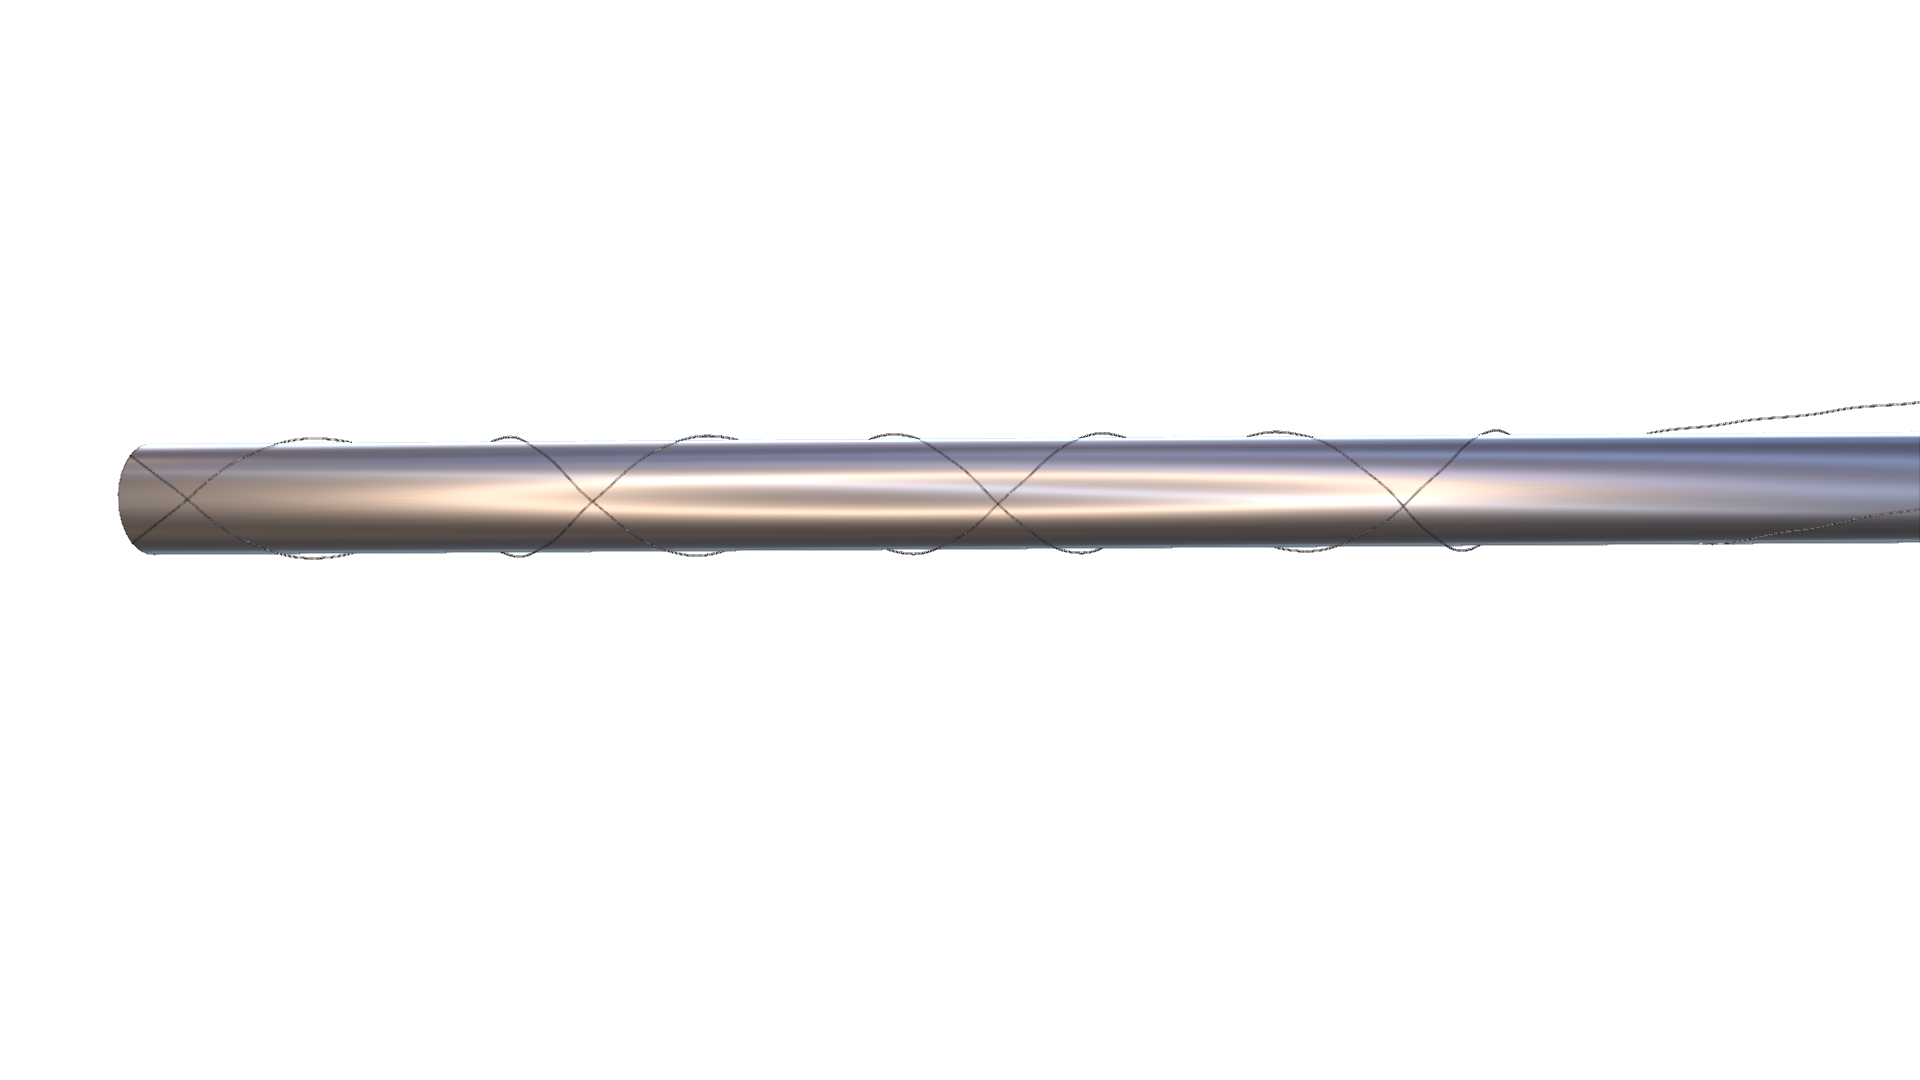
\includegraphics[width=400]{docs/figures/mortaryarnmandrel_1.png}
    \caption{Yarn-to-mandrel frictionless interactions modelled using mortar formulation for line contact (mandrel modelled as stocky beam).}
    \label{testsetup}
\end{figure}

















